\documentclass[12pt]{scrartcl}
\usepackage[english,ngerman]{babel} % Arbeit in DEUTSCHER SPRACHE % yes the order matters
\usepackage[utf8]{inputenc} % for Linux
\usepackage[numbers,square]{natbib}
\def\thesection{\arabic{section}}
\usepackage[official]{eurosym}
\usepackage{graphicx} % Required for inserting images
\usepackage{amsmath}
\usepackage{hyperref}
\usepackage{pdfpages}

\renewcommand{\sectionautorefname}{Kapitel}
\renewcommand{\tableautorefname}{Tabelle}

\begin{document}
\section{Notensystem der University of Technology Sydney (UTS)} 
\begin{table}[!ht]
    \centering
    \scalebox{1}{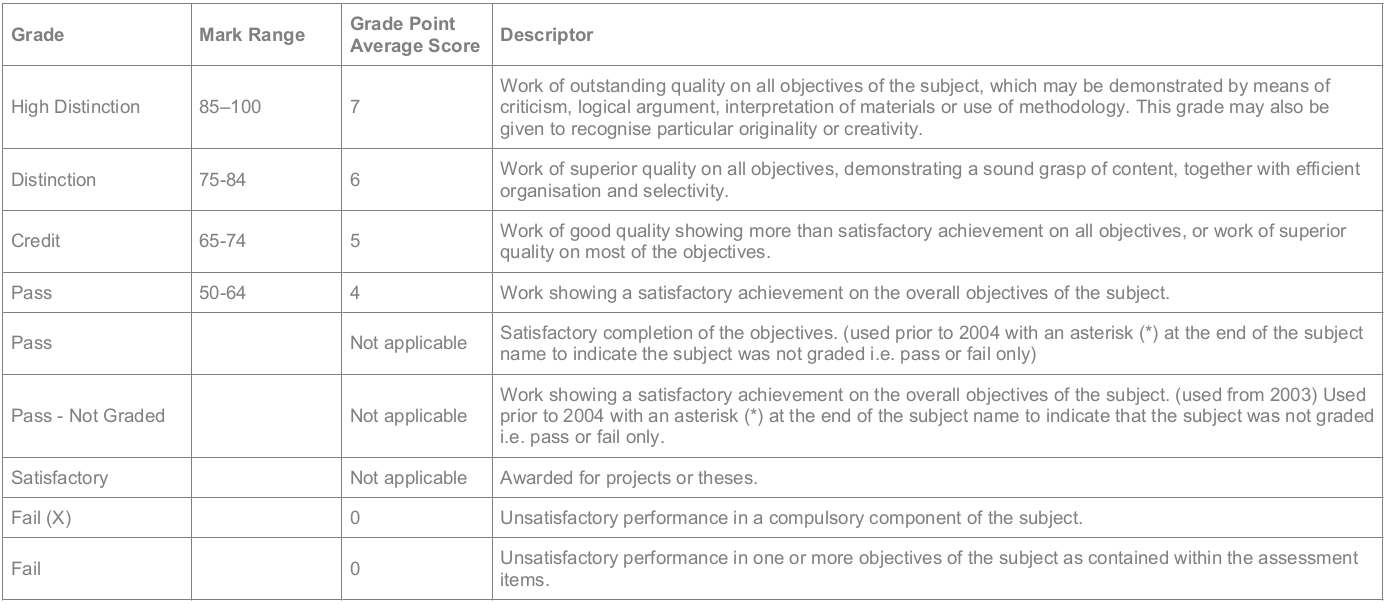
\includegraphics[width=\textwidth]{image.png}}
    \caption{Notentabelle UTS}
    \label{notentabelle}
\end{table}
Die Mark $M$ ist die durch den Studierenden erreichte Punktzahl $P$, als Anteil an der maximal möglichen Gesamtpunktzahl $G$. 

\begin{align*}
    M = \frac{P}{G}
\end{align*}

Beispielsweise gibt eine Mark von $78 \%$ an, dass der Student $78 \%$ der maximal zu erreichenden Gesamtpunktzahl erreicht hat. \\
Die Mark wird in eine Note (Grade) konvertiert, so, wie es in \autoref{notentabelle} angegeben ist. Eine Verwendung der Mark, als erreichte benotete Leistung, ist somit wenig zielführend. Dies wäre vergleichbar mit der Verwendung der prozentual erreichten Punktzahl in einer Klausur, als Maß für die erbrachte Leistung im Rahmen eines Vorlesungsmoduls, anstatt der gegebenen Note. \\
Aufgeführt wird ebenso ein zu der australischen Note äquivalenter GPA-Wert, welcher eine Angabe der australischen Note im, vor allem in den USA verwendeten, GPA-System ist. 
\newpage

\section{Bayerische Umrechnungsformel zur Umrechnung von ausländischen Noten}
Die bayerische Umrechnungsformel wird vom Hochschulbüro für Internationales der Leibniz Universität Hannover als verwendetes Maß zur Umrechnung ausländischer Noten angeführt. Sie bildet die Basis der Notenumrechnungstabelle. \cite{LUHNotenumrechnung}
\begin{align*}
    X &= 1 + 3 \left(\frac{N_{max}-N_d}{N_{max}-N_{min}}\right)\\[1ex]
    X &: \textrm{Umgerechnete Note}\\[0.5ex]
    N_{max} &: \textrm{Erreichbare Höchstnote}\\[0.5ex]
    N_{min} &: \textrm{Minimalnote zum Bestehen} \\[0.5ex]
    N_{d} &: \textrm{Zu übertragende Note}
\end{align*}

\section{Anwendung auf Notensystem der UTS}
Um die bayerische Umrechnungsformel auf das kategorische, nicht numerische, Notensystem der UTS anwenden zu können, muss den einzelnen Notenstufen ein numerischer Wert zugewiesen werden. Folgende Zuordnung scheint auf Basis von \autoref{notentabelle} sinnvoll:

\begin{gather*}
    \textrm{High Distinction} \; \widehat{=} \; 4\\
    \textrm{Distinction} \; \widehat{=} \; 3\\
    \textrm{Credit} \; \widehat{=} \; 2\\
    \textrm{Pass} \; \widehat{=} \; 1
\end{gather*}

Alternativ kann die Konvertierung aus \autoref{notentabelle} herangezogen werden, um die UTS-Note in einen GPA zu überführen.
Unabhängig von der gewählten Variante lässt sich nun die bayerische Umrechnungsformel anwenden.
\newpage

\section{Umrechnung Transcript of Records}
Die festgestellte Verfahrensweise soll für das in \autoref{transcript} aufgeführte Transcript of Records durchgeführt werden. Alle drei Fächer wurden mit der Note High Distinction abgeschlossen, sodass die Berechnung jeweils analog verläuft:

\begin{align*}
    X &= 1 + 3 \left(\frac{N_{max}-N_d}{N_{max}-N_{min}}\right)\\
      &= 1 + 3 \cdot \frac{4-4}{4-1} = 1 + 3 \cdot \frac{0}{3}\\ 
      &= 1,0 
\end{align*}

Dabei gilt $N_{max} = 4$, $N_d = 4$ und $N_{min} = 1$. Ähnlich verläuft die Berechnung unter Verwendung des GPA und der bayerischen Formel. Verwendet werden muss dann jedoch ein $N_{max}$ von $7$ bzw. $4$ und ein $N_{min}$ von $4$ bzw. $1$. \cite{LUHNotenumrechnung}\cite{GPA}\\
 Unter Berücksichtigung des GPA ist es ebenso möglich die Notenumrechnungstabelle heranzuziehen und die Notenkonversion aus den USA zu betrachten (\autoref{usa_gpa}). Wie in \cite{GPA} ersichtlich entspricht ein GPA von 7.0 aus dem neuen GPA-System einer 4.0 aus dem alten GPA-System. 
 \begin{table}[!ht]
 	\centering
 	\scalebox{1}{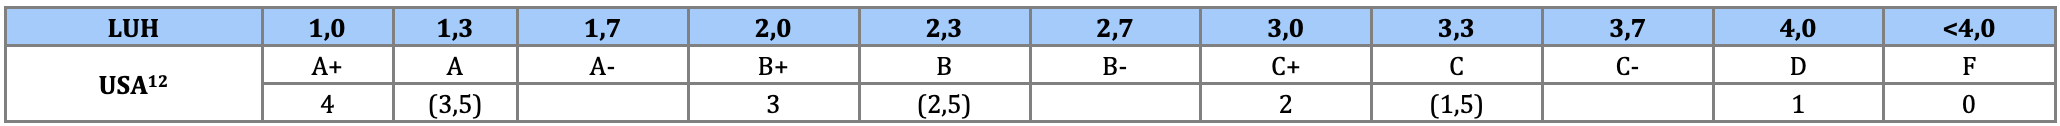
\includegraphics[width=\textwidth]{image2.png}}
 	\caption{Notenkonversion USA zu LUH}
 	\label{usa_gpa}
 \end{table}
 
 Unabhängig von der gewählten Methode konvertieren alle erbrachten Leistungen zu einer 1,0.
\newpage

\bibliography{ref}
\bibliographystyle{unsrt}
\newpage

\appendix
\pagenumbering{gobble}
\vspace*{\fill}
\hspace*{\fill}

\section{Transcript of Records Robert Zimmermann}
\label{transcript}

\hspace*{\fill}
\vspace*{\fill}

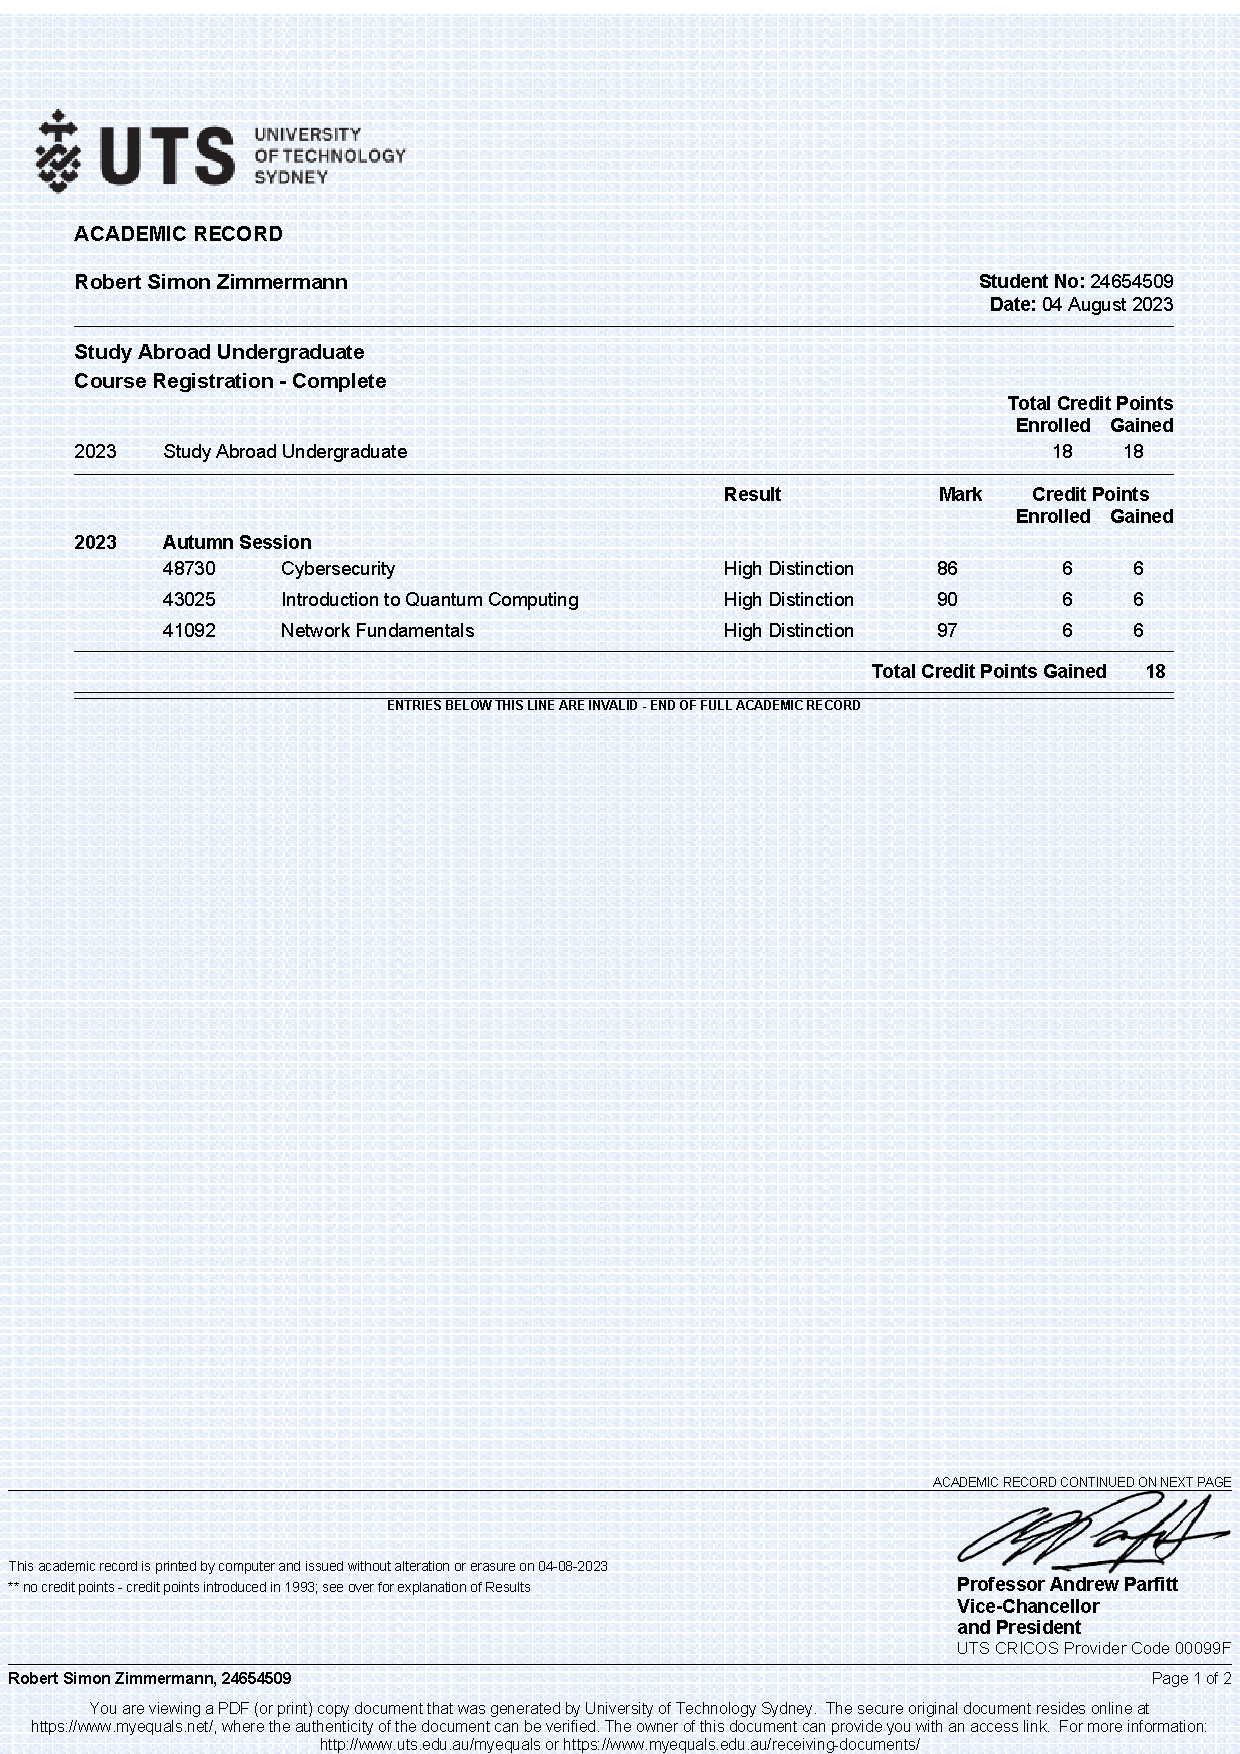
\includepdf[pages={1-},scale=0.95]{notenspiegel.pdf}
\label{bsp_anw}

\end{document}
